%% abtex2-modelo-trabalho-academico.tex, v-1.9.2 laurocesar
%% Copyright 2012-2014 by abnTeX2 group at http://abntex2.googlecode.com/ 
%%
%% This work may be distributed and/or modified under the
%% conditions of the LaTeX Project Public License, either version 1.3
%% of this license or (at your option) any later version.
%% The latest version of this license is in
%%   http://www.latex-project.org/lppl.txt
%% and version 1.3 or later is part of all distributions of LaTeX
%% version 2005/12/01 or later.
%%
%% This work has the LPPL maintenance status `maintained'.
%% 
%% The Current Maintainer of this work is the abnTeX2 team, led
%% by Lauro César Araujo. Further information are available on 
%% http://abntex2.googlecode.com/
%%
%% This work consists of the files abntex2-modelo-trabalho-academico.tex,
%% abntex2-modelo-include-comandos and abntex2-modelo-references.bib
%%

% ------------------------------------------------------------------------
% ------------------------------------------------------------------------
% abnTeX2: Modelo de Trabalho Academico (tese de doutorado, dissertacao de
% mestrado e trabalhos monograficos em geral) em conformidade com 
% ABNT NBR 14724:2011: Informacao e documentacao - Trabalhos academicos -
% Apresentacao
% ------------------------------------------------------------------------
% ------------------------------------------------------------------------

\documentclass[
	% -- opções da classe memoir --
	12pt,				% tamanho da fonte
	openright,			% capítulos começam em pág ímpar (insere página vazia caso preciso)
	twoside,			% para impressão em verso e anverso. Oposto a oneside
	a4paper,			% tamanho do papel. 
	% -- opções da classe abntex2 --
	%chapter=TITLE,		% títulos de capítulos convertidos em letras maiúsculas
	%section=TITLE,		% títulos de seções convertidos em letras maiúsculas
	%subsection=TITLE,	% títulos de subseções convertidos em letras maiúsculas
	%subsubsection=TITLE,% títulos de subsubseções convertidos em letras maiúsculas
	% -- opções do pacote babel --
	english,			% idioma adicional para hifenização
	french,				% idioma adicional para hifenização
	spanish,			% idioma adicional para hifenização
	brazil				% o último idioma é o principal do documento
	]{abntex2}

% ---
% Pacotes básicos 
% ---
\usepackage{lmodern}			% Usa a fonte Latin Modern			
\usepackage[T1]{fontenc}		% Selecao de codigos de fonte.
\usepackage[utf8]{inputenc}		% Codificacao do documento (conversão automática dos acentos)
\usepackage{lastpage}			% Usado pela Ficha catalográfica
\usepackage{indentfirst}		% Indenta o primeiro parágrafo de cada seção.
\usepackage{color}				% Controle das cores
\usepackage{graphicx}			% Inclusão de gráficos
\usepackage{microtype} 			% para melhorias de justificação
% ---
		
% ---
% Pacotes adicionais, usados apenas no âmbito do Modelo Canônico do abnteX2
% ---
\usepackage{lipsum}				% para geração de dummy text
% ---

% ---
% Pacotes de citações
% ---
\usepackage[brazilian,hyperpageref]{backref}	 % Paginas com as citações na bibl
\usepackage[alf]{abntex2cite}	% Citações padrão ABNT

% --- 
% CONFIGURAÇÕES DE PACOTES
% --- 

% ---
% Configurações do pacote backref
% Usado sem a opção hyperpageref de backref
\renewcommand{\backrefpagesname}{Citado na(s) página(s):~}
% Texto padrão antes do número das páginas
\renewcommand{\backref}{}
% Define os textos da citação
\renewcommand*{\backrefalt}[4]{
	\ifcase #1 %
		Nenhuma citação no texto.%
	\or
		Citado na página #2.%
	\else
		Citado #1 vezes nas páginas #2.%
	\fi}%
% ---

% ---
% Informações de dados para CAPA e FOLHA DE ROSTO
% ---
\titulo{Título de nosso TCC}
\autor{Higor Viana de Morais\and Josué Batista Matos Deschamps de Melo}
\local{São Paulo}
\data{2021}
\orientador{Clarice Gameiro da Fonseca Pachi}
\coorientador{Jorge Futoshi Yamamoto}
\instituicao{%
  Centro Universitário Senac - Santo Amaro
  \par
  Bacharelado em Ciência da Computação}
\tipotrabalho{Tese (Doutorado)}
% O preambulo deve conter o tipo do trabalho, o objetivo, 
% o nome da instituição e a área de concentração 
\preambulo{Monografia apresentada na disciplina Trabalho de Conclusão de Curso, como parte dosrequisitos para obtenção do título de Bacharelem Ciência da Computação}
% ---


% ---
% Configurações de aparência do PDF final

% alterando o aspecto da cor azul
\definecolor{blue}{RGB}{41,5,195}


% --- 

% --- 
% Espaçamentos entre linhas e parágrafos 
% --- 

% O tamanho do parágrafo é dado por:
\setlength{\parindent}{1.3cm}

% Controle do espaçamento entre um parágrafo e outro:
\setlength{\parskip}{0.2cm}  % tente também \onelineskip

% ---
% compila o indice
% ---
\makeindex
% ---

% ----
% Início do documento
% ----
\begin{document}

% Retira espaço extra obsoleto entre as frases.
\frenchspacing 

% ----------------------------------------------------------
% ELEMENTOS PRÉ-TEXTUAIS
% ----------------------------------------------------------
% \pretextual

% ---
% Capa
% ---
\imprimircapa
% ---

% ---
% Folha de rosto
% (o * indica que haverá a ficha bibliográfica)
% ---
\imprimirfolhaderosto*
% ---

% ---
% Inserir a ficha bibliografica
% ---

% Isto é um exemplo de Ficha Catalográfica, ou ``Dados internacionais de
% catalogação-na-publicação''. Você pode utilizar este modelo como referência. 
% Porém, provavelmente a biblioteca da sua universidade lhe fornecerá um PDF
% com a ficha catalográfica definitiva após a defesa do trabalho. Quando estiver
% com o documento, salve-o como PDF no diretório do seu projeto e substitua todo
% o conteúdo de implementação deste arquivo pelo comando abaixo:
%
% \begin{fichacatalografica}
%     \includepdf{fig_ficha_catalografica.pdf}
% \end{fichacatalografica}


% ---
% Inserir errata
% ---
%\begin{errata}
%Elemento opcional da %\citeonline[4.2.1.2]{NBR14724:2011}. Exemplo:

%\vspace{\onelineskip}

%FERRIGNO, C. R. A. \textbf{Tratamento de %neoplasias ósseas apendiculares com
%reimplantação de enxerto ósseo autólogo %autoclavado associado ao plasma
%rico em plaquetas}: estudo crítico na cirurgia de %preservação de membro em
%cães. 2011. 128 f. Tese (Livre-Docência) - %Faculdade de Medicina Veterinária e
%Zootecnia, Universidade de São Paulo, São Paulo, %2011.

%\begin{table}[htb]
%\center
%\footnotesize
%\begin{tabular}{|p{1.4cm}|p{1cm}|p{3cm}|p{3cm}|}
%  \hline
%   \textbf{Folha} & \textbf{Linha}  & \textbf{Onde se lê}  & \textbf{Leia-se}  \\
%    \hline
%    1 & 10 & auto-conclavo & autoconclavo\\
%   \hline
%\end{tabular}
%\end{table}

%\end{errata}
% ---

% ---
% Inserir folha de aprovação
% ---

% Isto é um exemplo de Folha de aprovação, elemento obrigatório da NBR
% 14724/2011 (seção 4.2.1.3). Você pode utilizar este modelo até a aprovação
% do trabalho. Após isso, substitua todo o conteúdo deste arquivo por uma
% imagem da página assinada pela banca com o comando abaixo:
%
% \includepdf{folhadeaprovacao_final.pdf}
%

% ---

% ---
% Dedicatória
% ---
%\begin{dedicatoria}
%   \vspace*{\fill}
%   \centering
%   \noindent
%   \textit{ Este trabalho é dedicado à.} \vspace*{\fill}
%\end{dedicatoria}
% ---

% ---
% Agradecimentos
% ---
\begin{agradecimentos}
Os agradecimentos principais são direcionados à Professora Doutora  Clarice Gameiro da Fonseca Pachi e ao Professor Doutor Jorge Futoshi Yamamoto que contribuíram para que a produção de trabalhos acadêmicos conforme as normas ABNT com \LaTeX\ fosse possível.

\end{agradecimentos}
% ---

% ---
% Epígrafe
% ---
%\begin{epigrafe}
%    \vspace*{\fill}
%	\begin{flushright}
%		\textit{``Não vos amoldeis às estruturas deste mundo, \\
%		mas transformai-vos pela renovação da mente, \\
%		a fim de distinguir qual é a vontade de Deus: \\
%		o que é bom, o que Lhe é agradável, o que é perfeito.\\
%		(Bíblia Sagrada, Romanos 12, 2)}
%	\end{flushright}
%\end{epigrafe}
% ---

% ---
% RESUMOS
% ---

% resumo em português
\setlength{\absparsep}{18pt} % ajusta o espaçamento dos parágrafos do resumo
\begin{resumo}
Ao abordar conceitos matemáticos e computacionais é possível analisar a transmissão de dados na rede de computadores de um complexo como o Hospital das Clínicas da Faculdade
de Medicina da Universidade de São Paulo (HCFMUSP).

Ao investigar o fluxo de dados na rede de computadores do HCFMUSP será viável explorar, principalmente, o tráfego de imagens médicas, considerando todas as conexões com os equipamentos que permitem o fluxo os dados.

O objetivo é examinar os modelos matemáticos que melhor representem as séries temporais geradas pelo tráfego na rede e, por meio do uso da linguagem Python uma das ferramentas computacionais associadas, gerar gráficos e fazer predições úteis para melhorar o fluxo de dados em um complexo hospitalar.

\textbf{Palavras-chaves}: Séries Temporais, Rede de Computadores, Imagens Médicas, Python.
\end{resumo}

% resumo em inglês
\begin{resumo}[Abstract]
 \begin{otherlanguage*}{english}
In this work, we study mathematical and computational concepts to understand and analyze data transmission in the network of the Hospital das Clínicas complex of the Faculty of Medicine of the University of São Paulo (HCFMUSP).

Studying the data flow within the HCFMUSP computer network we investigate, mainly, the traffic of medical images, considering all the connections with the equipment that support the data flow.

Our objective is to study the mathematical models that adequately represent the time series generated by traffic in this network and, through Python language and other associated computational tools, generate graphs and make useful predictions better understand the data flow in this hospital complex.

   \vspace{\onelineskip}
 
   \noindent 
   \textbf{Key-words}: Time Series, Computer Network, Medical Images, Python.
 \end{otherlanguage*}
\end{resumo}

% ---

% ---
% inserir lista de ilustrações
% ---
\pdfbookmark[0]{\listfigurename}{lof}

\listoffigures*
\cleardoublepage
% ---

% ---
% inserir lista de tabelas
% ---
\pdfbookmark[0]{\listtablename}{lot}
\listoftables*
\cleardoublepage
% ---

% ---
% inserir lista de abreviaturas e siglas
% ---
\begin{siglas}
\item[ARIMA] Auto Regressive Integrated Moving Average
\item[AR] Auto Regressão
\item[ACR] American College of Radiology
\item[DICOM] Digital Imaging and Communications in Medicine
\item[ed.] Edição
\item[HC] Hospital das Clínicas
\item[HCFMUSP] Hospital das Clínicas Faculdade de Medicina da Universidade de São Paulo
\item[HTTP] Hypertext Transfer Protocol 
\item[IP] Internet Protocol
\item[NEMA] National Electrical Manufacturers Association
\item[MM] Médias Moveis
\item[MBS] Medicare Benefits Program
\item[NETI] Núcleo Especializado de Tecnologia da Informação
\item[NETI – HCFMUSP] Núcleo Especializado de Tecnologia da Informação Hospital das Clínicas da Faculdade de Medicina da Universidade de São Paulo
\item[OSI] Open System Interconnection
\item[PACS] Picture Archiving and Communication System
\item[RPA] Robotic Process Automation
\item[SARIMA] Modelo Autorregressivo Integrado de Média Móvel Sazonal
\item[SFlow] Sample Flow
\item[TCP] Transmission Control Protocol
\end{siglas}
% ---

% ---
% inserir lista de símbolos
% ---
\begin{simbolos}
  \item[$ \Gamma $] Letra grega Gama
  \item[$ \Lambda $] Lambda
  \item[$ \zeta $] Letra grega minúscula zeta
  \item[$ \in $] Pertence
\end{simbolos}
% ---

% ---
% inserir o sumario
% ---
\pdfbookmark[0]{\contentsname}{toc}
\tableofcontents*
\cleardoublepage
% ---



% ----------------------------------------------------------
% ELEMENTOS TEXTUAIS
% ----------------------------------------------------------
\textual

% ----------------------------------------------------------
% Introdução (exemplo de capítulo sem numeração, mas presente no Sumário)
% ----------------------------------------------------------
%\chapter*[Introdução]{Introdução}
%\addcontentsline{toc}{chapter}{Introdução}
\chapter{Introdução}
% ----------------------------------------------------------

Com o grande volume de dados disponíveis no tráfego da internet, é necessário cada vez mais a coleta e a análise contínua de bilhões de dados. A mineração desses dados tem requisitado modernas e eficazes infraestruturas distribuídas que possam suportar o processamento desses \emph{Big Data} (BARROSO%% HÖLZLE, 2009).

A evolução das tecnologias de transmissão permitiu que as redes de computadores troquem informações em larga escala e com velocidade compatível com as necessidades de uma sociedade da informação e da comunicação de dados. Dessa forma, as questões relacionadas a infraestrutura ganharam destaque e passaram a interessar aos gestores de diversas áreas (COMER, 2007).

As redes de computadores permitem enviar informações como imagens, sons, vídeos e muitos tipos de arquivos. Essa transmissão pode ser usada para vários fins, incluindo a transmissão de imagens médicas, usando tecnologias específicas como o \emph{DICOM (Digital Imaging and Communications in Medicine)} e o \emph{PACS (Picture Archiving and Communication System)} entre outras.

É exploradas as características dos dados relacionados as imagens médicas que são obtidas e armazenadas no \emph{PACS} e transmitidas pela rede \emph{TCP/IP} existente em grandes complexos, obedecendo ao protocolo denominado \emph{DICOM}.

As imagens médicas têm como objetivo permitir que os profissionais de saúde visualizem o corpo humano internamente e de forma não invasiva, a fim de tornar o diagnóstico mais preciso. A tecnologia de raio X existe desde o início do século XIX e a imagem médica 
tridimensional apareceu em 1972 com a invenção da tomografia computadorizada (YOO, 2004).

Há protocolos que permitem a integração entre diferentes sistemas de obtenção de imagens médicas e o mais conhecido é o \emph{HL7 (Health Level 7)}, que permite a troca de informações entre o sistema de informações de pacientes e o DICOM, material de estudo desse trabalho (PIANYKH, 2012).

O  \emph{DICOM} é um sistema de comunicação para imagens digitais na medicina, que, tem como representação uma série de regras criadas em 1983 no  \emph{American College of Radiology}, que visam facilitar a armazenagem e comunicação de imagens. Desde sua criação, já sofreu três alterações para que houvesse uma melhoria no sistema de imagens e melhor expansão do  \emph{PACS} para conversação com sistemas e versões diferentes, melhorando a experiência e acesso para profissionais visualizarem exames em qualquer dispositivo (PIANYKH, 2012).

O PACs é um tipo de tecnologia que facilita a comunicação e arquivamento de clínicas diagnósticas através de estudos por imagens. Trata-se de uma ferramenta muito útil para evitar a perda de laudos, redução de custos e possibilita uma melhor flexibilidade dos dados armazenados (STRICKLAND, 2000).

Nesse contexto, surgiu a proposta em parceria com o NETI - HCFMUSP (Núcleo Especializado de Tecnologia da Informação Hospital das Clínicas da Faculdade de Medicina da Universidade de São Paulo), que por meio de ferramentas de código aberto, visa analisar o fluxo de dados da rede de computadores dessa instituição pública.

\section{Justificativa}

Considerado um dos mais importantes polos brasileiros de disseminação de informações técnico-científicas, o HCFMUSP é um Centro de excelência e referência no campo de ensino, pesquisa e assistência.

Com área construída de cerca de 380 mil metros quadrados, conta com dois mil leitos e 15 mil profissionais nas mais diversas atividades. É formado por sete institutos, dois hospitais auxiliares, laboratórios de investigação médica, unidades especializadas e demais áreas de apoio como o Prédio da Administração e Anexos, o Centro de Convenções Rebouças e a Escola de Educação Permanente.

Em relação ao parque tecnológico, o HCFMUSP dispõe de um total de máquinas em torno de 9000 computadores distribuídos entre os usuários, além de alguns data centers, sendo que o principal está localizado em um ponto central do complexo hospitalar, com diversas fibras óticas em topologia de estrela-anel interligando todos os institutos. 

Diante da complexidade dessa rede e do volume de tráfego do HCFMUSP, pode-se destacar a importância de se manter um sistema íntegro e funcional que evite falhas que comprometam a integridade dos dados (PACHI et al., 2021).

Existem muitas soluções exclusivas para ajudar nas tarefas de análise de tráfego de redes de computador. Em geral, essas ferramentas permitem coletar e armazenar dados para análise em tempo real e posterior. Ao usar essas ferramentas em pontos estratégicos de uma rede é possível capturar dados globais ou fragmentados, dependendo de suas necessidades analíticas. Portanto, fazer a escolha de um ponto de coleta de tráfego é fator essencial para projetos de análise de rede e, conforme a rede cresce, a tarefa de coletar dados de tráfego se torna cada vez mais complexa (MACEDO, 2015).

Atualmente o mundo todo lida com diversos tipos de informações que são espalhadas através da internet. Com isso a tecnologia para coleta e análise de dados ganha um espaço importante em grande parte das empresas, permitindo que a informação seja obtida, armazenada, compartilhada e visualizada de forma mais otimizada.

A exploração do tráfego de dados dentro de um complexo hospitalar ganha relevância ao entender como funciona o processo de transferência de dados, quais as medidas de segurança para que os dados transmitidos não sejam expostos e como eles poderão ajudar aquele que irá analisá-los.

Assim, ao explorar o fluxo de dados dentro da rede de computadores do HCFMUSP facilita descrever o tráfego de imagens médicas dessa rede, considerando todas as conexões dos com os equipamentos que permitem o fluxo dos dados de armazenamento e do Input/Output dos servidores PACS, ainda sendo importante analisar o fluxo de dados dos switches que fazem a transmissão dos dados por meio do protocolo SFlow.

Com os resultados gerados, uma investigação dos modelos de séries temporais mais apropriados para descrever essa rede é necessário, sendo considerado o modelo ARIMA para ajustar modelos autorregressivos integrados de médias móveis, pois com este modelo torna-se mais prático e preciso fazer análises por conta do uso de Médias Móveis e Autorregressão.

\section{Objetivos}

Investigar o tráfego de rede no complexo HCFMUSP, verificando o fluxo de dados e utilizando séries temporais com uso de linguagem de programação para analisar comportamentos do presente e do futuro. 

\section{Objetivos Específicos}

\begin{quote}
•	Facilitar as análises periódicas e/ou com uma ferramenta de apoio;
\end{quote}
\begin{quote}
•	Estudar os melhores modelos matemáticos que representem o comportamento dessa rede;
\end{quote}
\begin{quote}
•	Usar a ferramenta de desmembramento de informações UiPath (pago, usado como teste), Repl.it e Google Colab (ambas gratuitas e online) para desenvolver uma prototipagem;
\end{quote}
\begin{quote}
•	Utilizar linguagem de programação com os modelos matemáticos estudados para desenvolver o código.
\end{quote}


% ---
% Capitulo com exemplos de comandos inseridos de arquivo externo 
% ---
%\include{abntex2-modelo-include-comandos}
% ---

% ----------------------------------------------------------
% PARTE
% ----------------------------------------------------------
%\part{Referenciais teóricos}
% ----------------------------------------------------------

% ---
% Capitulo de revisão de literatura
% ---
\chapter{Revisão de Literatura}
% ---

% ---
\section{Imagens médicas}

O corpo humano é complexo para a compreensão, por isso que para estudá-lo são usadas as imagens médicas que são formas de obter e revelar dados de forma simples para humanos. Essas imagens estão sempre relacionadas a qualquer tipo de interação de um determinado tipo de energia (eletromagnética, mecânica) com a matéria. A imagem é visualizada por meio de um parâmetro de contraste, determinado por algumas propriedades físicas que distinguem diferentes tecidos, órgãos ou sistemas. Com exceção do ultrassom, que usa energia e mecânica, a maioria das imagens médicas tem uma interação entre a energia eletromagnética e o corpo humano (SILVA; PATROCÍNIO; SCHIABEL, 2019).

Várias evoluções ocorreram durante a história da medicina, para que no século XXI, a tecnologia permitisse que as imagens médicas pudessem ser utilizadas com os recursos que são dispostos. É possível dizer que a descoberta do raio X no século XIX iniciou uma história que chegou até hoje com constantes evoluções das serão analisadas. 

\begin{quote}
''No dia 8 de novembro de 1895, Wilhelm Conrad Rõntgen, então professor de física na Universidade de Würzburg, Bavária, Alemanha, descobre uma nova espécie de radiação produzida pela passagem de uma corrente elétrica por um tubo de vidro sob vácuo, e que possuia a singular qualidade de, embora invisível a olho nu, produzir fluorescência ao incidir sobre um papel impregnado por cianureto de bário e platina. Mais impressionante era a capacidade destes raios de atravessar corpos sólidos (madeira, papel, partes do corpo humano), com maior ou menor intensidade, dependendo da natureza do material''% \cite{ARRUDA, 1996, p. 1}.
\end{quote}

Após o descobrimento da Radiologia, pode-se visualizar que a Radioatividade estava para ganhar seu espaço no mundo. Em 1896 estudos sobre ela ganharam vida após a descoberta que mudaria a história, estudo este atribuído às descobertas feitas por Henri Becquerel, mas que na verdade, a principal contribuição foi de Marie Curie com a descoberta dos materiais radioativos que conhecemos hoje: tório, rádio polônio, em 1898. Esta contribuição foi dada como um prefácio ao Beckerell, pois a descoberta da radiação do urânio seria "natural" para encontrar outros elementos que emitam o mesmo tipo de radiação. (MARTINS, 2003)

%%CITAÇÃO AQUI

Com estas descobertas mesmo sendo perigosa se não usada da maneira adequada, a radioatividade tomou um lugar essencial na medicina, pois doenças puderam ser diagnosticas com mais eficiência e rapidez. Em alguns casos até mesmo tratamentos que poderiam ser impossíveis se tornaram possíveis. (CARVALHO, 2015)

Desse modo a medicina ganhava um novo aspecto se tornando mais confiável e cada vez mais evoluindo seus métodos. Pode-se notar isso também com o uso da Radiologia, que com o passar dos anos também foi tomando forma no meio hospitalar.

As imagens analógicas por anos desempenharam um papel importante na sociedade, mas como não só a medicina tomou este rumo evolutivo, assim outras tecnologias também surgiram, tornando o mundo cada vez mais globalizado. Isso faz com que algumas tecnologias se tornem “ultrapassadas” não sendo mais tão eficientes como antes. E com isso surgem as imagens médicas digitais (FILHO; XAVIER; ADRIANO, 2001)

Dessa forma a evolução tecnológica do radiodiagnóstico tomou um rumo interessante, onde atualmente com o uso da tecnologia da informação, diversos hospitais adotam medidas que facilitam o trabalho e minimizam custos administrativo, mas para isso deve-se entender que estes métodos possuem os chamados protocolos, que são essenciais no funcionamento dessas ferramentas tecnológicas (FILHO; XAVIER; ADRIANO, 2001).

% ---
\section{Protocolos}
% ---
Protocolos são meios de comunicação que transmitem informações bem definidas para execução de tarefas. São usados por diversos computadores em uma rede, fazendo assim com que todos possam usar os mesmos protocolos para que a comunicação ocorra de forma eficaz. (RIOS, 2012)

Existem vários tipos de protocolos, como por exemplo \emph{FTP}, \emph{FMTP}, \emph{TDS}, \emph{SBM}, \emph{SSH}, \emph{DNS} e um importante protocolo usado no monitoramento de transmissão de dados do HCFMUSP, o \emph{Sflow}.

\begin{quote}
''Paralelo ao NetFlow e ao IPFIX, o protocolo sFlow surge como alternativa para o monitoramento baseado em ambientes de volume de tráfego extremamente altos pois diferentemente do método de agregação do fluxo de tráfego utilizado pelo NetFlow e consequentemente pelo IPFIX, o protocolo sFlow utiliza um método flexível de amostragem que garante alta performance na elaboração dos fluxos visto não necessitar analisar todo o tráfego para gerar as informações estatísticas conforme descrito em (PHAAL, PANCHEN, %& MCKEE, 2001). (COUTO, 2012)'' \cite{ARRUDA, 1996, p. 1}.
''
\end{quote}

Dentre todos os esses o chamado Transmission Control Protocol (TCP) que é unificado em seu uso com o Internet Protocol (IP), formando assim o TCP/IP, no qual surgiu em meados de 1960. (RIOS, 2012)

O modelo TCP/IP vem justamente do conceito de controlar a transmissão dos dados de uma rede, ou seja, garantir que haverá uma comunicação entre máquinas. Ele é dividido em camadas que desempenham um papel importante nessa transmissão, que são: Aplicação, que garante a visualização de dados para um humano, muita das vezes usando protocolos como Hypertext Transfer Protocol ou Protocolo de Transferência de Hipertexto (HTTP); Transporte, que garante a organização dos dados recebidos e fazer a ponte que liga duas comunicações; Inter-rede, que justamente determina o endereço do computador através do IP; host/rede, que recebe os dados enviados pela inter-rede e fará controle e correção de erros na transmissão dos dados envolvidos na rede. (RIOS, 2012)

Esses protocolos são fundamentais para transmissão de dados e no caso das imagens ganham uma grande importância, pois para hospitais toda a rotina clínica se torna fácil, e principalmente no HCFMUSP, onde o volume de transmissão de dados de imagens médicas representam aproximadamente 600 mil imagens por dia. 

\subsection{DICOM}

Desde o surgimento de exames por imagem a forma com que as informações eram armazenadas e visualizadas foram evoluindo de maneira que o American College of Radiology (ACR) e a National Electrical Manufacturers Association (NEMA), notaram o quão importante seria manter padrões para transferência da dados de imagens médicas (REGERT; PRÜSSE, 2005).

Com isso, em 1983 reuniram-se pessoas para elaborarem um padrão para este tipo de comunicação digital, que em 1985 ganhou forma e foi então criado o DICOM, que é uma linguagem usada como padrão para gerenciar informações através do tráfego de redes de computadores, facilitando a radiologia (REGERT; PRÜSSE, 2005).

Com o passar dos anos o DICOM passou por 2 mudanças, tendo a sua primeira versão em 1895 chamada de ACR-NEMA 300-1985 ou ACRNEMA 1.0, a segunda chamada ACR-NEMA 300-1988 ou ACRNEMA-2.0 e a usada desde 1993 a ACR-NEMA DICOM ou DICOM-3.0 (ROGALSKY, 2017).

\begin{quote}
''[...] aplicada a um ambiente em rede e à troca de mídia off-line, definindo o formato do arquivo e dando suporte a vários tipos de mídias físicas. Além disso, é um protocolo orientado para o serviço, que especifica a semântica de comandos e dados associados, e como os dispositivos reagem a comandos e transferência de dados. Sendo assim, inclui suporte para gerenciamento do fluxo de trabalho de um departamento de imagens e explicitamente descreve como um programador deve estruturar a Declaração de Conformidade para seleção de opções específicas. (ROGALSKY, 2017, p. 2)''
\end{quote}

\subsection{PACS}

\begin{quote}
''A partir da década de 1980, o gerenciamento de imagens médicas segue uma padronização chamada PACS (Picture Archiving and Communication System) ou sistemas de arquivamento e comunicação de imagens (MARSH, 1997). Estes sistemas permitiram o armazenamento e recuperação das imagens médicas em uma rede de computadores que propiciaram uma grande coleção de imagens armazenadas em banco de dados (OLIVEIRA, 2012, p. 15).''\end{quote}

Embora existam centenas de instalações de PACS em todo o mundo, muitas são apenas pequenas, como conectar uma unidade de terapia intensiva a uma unidade de radiologia ou conectar algumas estações de trabalho em rede, e é questionável se esses sistemas merecem o nome de PACS. (STRICKLAND, 2000)

Uma vez que a imagem é armazenada pelo PACS há a garantia de que ela não será violada ou perdida, tendo assim uma disponibilidade altíssima, já que permite visualização simultânea em diversos pontos do hospital, por conta dos numerosos terminais instalados em todo o hospital, e uma grande flexibilidade em qualquer lugar do hospital para executar decisões clínicas de forma coerente e sem que haja conflito entre dados de vários pacientes. Com isso todas as imagens serão organizadas em grupos que mantem uma ordem cronológica e nomeada de acordo com o paciente em questão, graças ao seu banco de dados. (STRICKLAND, 2000)

Ainda é possível considerar o fator econômico, pois de forma direta o PACS garante um custo-benefício enorme, eliminando o esforço de uma Radiologia com filme, uso de produtos químicos para o processo de visualização, salários para funcionários de câmera escura e arquivistas de filme e espaço físico para armazenar as imagens obtidas. Embora seja possível considerar todos estes benefícios, ainda deve-se considerar que os técnicos de câmara escura serão substituídos por funcionários de Tecnologia da Informação (STRICKLAND, 2000).

\section{Estatísticas Descritivas}

Coletar, analisar e interpretar dados são necessidades para qualquer ser humano. Por este motivo a Estatística Descritiva desempenha um importante papel nesta situação, pois nela é utilizado os dados coletados para serem analisados em gráficos e diagramas que posteriormente trará informações acerca do que se busca.

Para entendimento de como a Estatística Descritiva funciona, deve-se saber a diferença entre inferência dedutiva e inferência indutiva. A dedutiva se trata de usar lógica para obter conclusões com o ponto inicial da análise, já a indutiva trata-se de generalizar os dados, fazendo análises e várias conclusões possível. Neste caso será abordado apenas a indutiva.

Com a inferência indutiva pode-se estabelecer conceitos que facilitam a compreensão para realiza-se a pesquisa necessária, que são: 

•	População: público-alvo de pessoas ou elementos que são estudados que bem a represente;

•	Amostra: uma fração da população;

•	Parâmetro: usado para a população;

•	Estimativa: usado para a amostra, para estimar um parâmetro.

•	Variável: é uma característica da população, onde com ela pode-se determinar qual o tipo de coleta/análise será feita. Esta possui 4 categorias, das quais são:

o	Variável Qualitativa Nominal: os valores não são numéricos e não necessitam de uma hierarquia. Ex.: qual o modelo ou nome de um computador em uma rede hospitalar.

o	Variável Qualitativa Ordinal: os valores não são numéricos e respeitam uma hierarquia entre si. Ex.: qualidade de conexão para a internet, ótima, boa, ruim, péssima.

o	Variável Quantitativa Discreta: os valores são numéricos inteiros, ou seja, valores que fazem parte de uma contagem. Ex.: número de computadores em um hospital.

o	Variável Quantitativa Contínua: os valores são numéricos reais, ou seja, qualquer número possível. Ex.: quantidade de tempo em que uma máquina se comunica com a outra através da rede.

Sabendo dessas informações pode-se construir gráficos a fim de mostrar de forma visual como os dados de uma variável quantitativa se comportam. Na Figura 1 é possível verificar a quantidade de vezes em que alguns protocolos foram utilizados em transmissões de dados da rede hospitalar.

% --- FIGURA ---

\begin{figure}[htbp]
\hypertarget{arquitetura}{%
\caption{Alguns protocolos da rede do HCFMUSP}\label{arquitetura}
\begin{center}
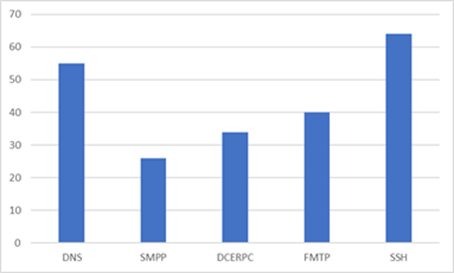
\includegraphics{Figuras/Figura 1 - Alguns protocolos da rede do HCFMUSP.png}
\end{center}
}
\legend{Fonte: Elaborado pelo(a) autor(a).}
\end{figure}

% --- FIGURA ---

Além de visualizar os dados de variável quantitativa, é possível manipulá-los com o uso das medidas de posição dentro da amostra, que são:

•	Moda: um determinado valor que aparece mais vezes do que os demais valores na amostra coletada. Em geral a moda é usada em casos em que existem variáveis quantitativas discretas;

•	Média: se trata de calcular um valor geral para uma amostra, ou seja, soma-se todos os elementos da amostra, x1, x2, ..., xn. 

Depois é divido a soma pela quantidade total n de uma determinada amostra. Assim é obtido um valor que será denominado a média de uma amostra

•	Mediana: trata-se de organizar os valores encontrados na amostra e ordená-los de maneira que seja encontrado um valor central. Por exemplo, uma sequência com os valores: 4, 7, 8, 12, 3, 12, 5; deverá ser ordenada de forma que o valor central da sequência possa aparecer: 3, 4, 5, 7, 8, 12, 12. Neste caso com uma quantidade ímpar de valores é facilmente encontrado o valor central, mas quando se tem uma quantidade par, precisa-se obter os 2 valores centrais, somá-los e dividi-los por 2. Dessa forma é encontrada a mediana através da média formada por estes 2 valores centrais.

Além das medidas de posição existem também as medidas de dispersão, pois nem sempre as medidas de posição serão suficientes. Trata-se de calcular os valores da amostra e sua média, ou seja, quanto menor a distância destes, a variável será mais homogênea, caso contrário, mais heterogênea. Para isso estuda-se 3 tipos de medidas, que são:

•	Desvio médio: uma amostra possui n variáveis que podem ser manipuladas calculando a soma dos desvios absolutos. Estes desvios representam a diferença entre um elemento x da amostra e a média dessa amostra. Da mesma forma que o cálculo da média, quando se soma todos os desvios absolutos, deve-se dividi-los pela quantidade n de elementos. Este resultado será o desvio médio;

•	Variância: Se tem algo parecido com o desvio médio, mas ao em vez de usar apenas o desvio absoluto, é feito com que ele seja quadrático, ou seja, o desvio absoluto elevado a 2. Dessa forma é garantido que os desvios absolutos mantenham um valor natural (maior que 0). Por fim basta apenas dividir a soma total pela quantidade n de elementos;

•	Desvio padrão: Para que possa manter uma unidade equivalente a original, basta utilizar a raiz quadrada na variância que é encontrada como método. Com isso pode-se determinar que quanto menor o desvio padrão, a variável será mais homogênea.

Sabendo agora acerca do desvio padrão, é possível entender como o erro padrão funciona. Apesar dos nomes parecidos, eles se diferem quanto ao seu uso, pois como o próprio nome diz, deseja-se encontrar o erro nesta amostra, ou seja, o erro padrão é uma aproximação do desvio padrão das médias encontradas na amostra. Para calcular basta apenas dividir o desvio padrão pela raiz quadrada do número total de elementos em uma amostra. (LUNET; SEVERO; BARROS, 2006).

% ---
\section{Séries Temporais}
% ---

A série temporal é uma série de observações organizadas em ordem cronológica. Por exemplo, se tem um experimento em que uma determinada variável é coletada semanalmente, mensalmente ou anualmente, tem uma série temporal indexada para esse período, independentemente de ele ser um fator importante na pesquisa cronológica. Cada curva formada por uma série recebe o nome de trajetória do processo físico e o que se chama de série temporal é uma parte da trajetória (MORETTIN%&TOLOI, 2006).

Do ponto de vista estatístico, é possível dizer que uma série temporal é a realização de um processo estocástico ordenado em intervalos regulares de tempo. 

Os dados de uma série temporal geralmente não são independentes, especialmente se os intervalos da amostra são curtos. Pode-se concluir que as observações próximas costumam ser mais que parecidas com os dados reais da série do que os dados posicionados mais distantes dos dados originais. 

Ao considerar a ordem temporal, as séries podem ser classificadas como discretas ou contínuas. No primeiro caso as observações são obtidas em intervalos de tempo discretos e equidistantes, já nas séries contínuas observações são obtidas em qualquer intervalo de tempo (MORETTIN%&TOLOI, 2006).

A análise de uma série temporal permite entender o comportamento histórico de uma série e fazer previsões com base nessa história. Isso permite por exemplo, prever a demanda de ações do mercado financeiro e, embora o preço de uma ação seja afetado por muitos fatores externos, ainda assim é possível fazer estimativas econômicas. A Figura 2 mostra a umidade mínima e média em Manaus em maio de 2021.

\subsection{Tendência}

A tendência é a diferença entre a medida média e o valor de referência da medida, criada pelo avaliador utilizando o mesmo equipamento e método. Ou seja, é responsável por alterar o primeiro momento da distribuição conjunta do processo estocástico em questão e influenciar a média do processo (Macedo, 2015). 

A Figura 5 apresenta dados sobre a COVID-19 registrados no Rio Grande do Norte durante o período de 18 de março de 2020 a 14 de setembro de 2020 extraídos pela linguagem Python, mostrando uma tendência de decaimento.


\subsection{Estacionariedade}

Uma série temporal é considerada estacionária se ocorrer aleatoriamente no tempo em torno de uma média constante. Isso reflete alguma forma de equilíbrio estável. A distribuição das articulações não muda com o tempo de viagem. Esta é a forma mais forte de estacionariedade. Na verdade, a maioria das séries que se encontra mostra algum tipo de não-estacionariedade, como tendências (MACEDO, 2015).

A série pode ser estacionária por curtos ou longos períodos. Isso significa uma mudança no nível e/ou inclinação. A classe do modelo ARIMA, por exemplo, é suficiente para descrever sequências estacionárias e não estacionárias que não exibem comportamento explosivo. Este tipo de não estacionariedade ocorre quando a sequência é estacionária, flutuando em torno de um determinado nível de tempo, mudando de nível e flutuando em torno de um novo nível, ou quando o gradiente pode ser alterado (MACEDO, 2015).

A maioria dos procedimentos de análise estatística de séries temporais pressupõe que são estacionários. Portanto, se não formar uma série estacionária, precisará transformar os dados originais. A transformação mais comum é obter a derivada da série original até obter a série estacionária (MACEDO, 2015). A Figura 6 mostra o processo estacionário de vendas de veículos.

\subsection{Sazonalidade}

A sazonalidade se refere às estações, ou seja, eles sempre ocorrem em um momento específico. Na área de negócios, a sazonalidade é um termo relacionado a fatores externos que se repetem ao longo do tempo e podem afetar o desempenho de uma empresa. Essas variações sazonais podem ter várias causas, incluindo clima (estações do ano), eventos (Carnaval, Copa do Mundo) e datas comemorativas (Dia das Mães, Natal). (MACEDO, 2015). Existem dois tipos de sazonalidade:

•	Sazonalidade determinística: O coeficiente de cada variável representa o fator sazonal do respectivo mês, trimestre etc.;

•	Sazonalidade estocástica: Variável com defasagem sazonal no modelo (modelos ARMA periódicos ou modelo ARMA sazonal).

A Figura 7 mostra dados de pacientes, que compraram medicamentos para diabetes na Austrália entre 1992 e 2008.

Nas redes de computadores, a sazonalidade costuma não ser determinística, mas é possível especificar um período recorrente, como no caso dos finais de semana, quando a rede é subutilizada por diversos aplicativos (MACEDO, 2015).

\subsection{Autocorrelação}

Em matemática, um objeto de autocorrelação é exatamente ou aproximadamente semelhante a uma parte de si mesmo. Muitos objetos no mundo real, como litorais continentais, são estatisticamente semelhantes. Ou seja, alguns deles têm as mesmas propriedades em escalas diferentes. A autossimilaridade é uma característica típica dos fractais, por exemplo (MACEDO, 2015).

A autossimilaridade é uma ideia antiga, uma propriedade geométrica simples. É "simetria entre escalas". Ou seja, um objeto é semelhante a si mesmo se exibir a mesma forma em qualquer escala observada, embora nem todos os objetos geométricos têm essa propriedade. Matematicamente, as características de autossimilaridade são descritas por transformações nas quais as imagens dos objetos são suas "cópias reduzidas". Essas transformações são chamadas de transformações similares (MACEDO, 2015).

O objetivo da análise de uma série temporal consiste em elaborar um modelo estatístico que descreva adequadamente a procedência de uma série dados, de forma que as implicações teóricas do modelo sejam compatíveis com as amostras observadas nas séries temporais. A Figura 8 mostra a autocorrelação entre uma ação da Tesla de 250 dias e seu preço.

O modelo elaborado a partir da série temporal pode ser utilizado para prever a evolução futura da série ou explicar a relação entre os distintos componentes do modelo.

% ---
\section{Modelos Matemáticos}

Existem diversos tipos de modelos matemáticos e eles são cruciais para que o desenvolvimento de estudos das séries temporais. Alguns modelos que normalmente tem uma aplicação no estudo de redes de computadores serão abordados nos próximos tópicos.

% ---

\subsection{Modelo de Poisson}

Também denominado como Distribuição de Poisson, trata-se de um modelo proposto por Siméon Denis Poisson, onde em seu livro Recherches seve la probabilité de jugements en matière criminelle et en matière civile publicado em 1837 explica conceitos probabilísticos envolvendo principalmente questões judiciais, mas que também possui uma ampla aplicação em várias áreas, bem como a aproximação de variáveis aleatórias binomiais. (BARBOSA, 2014)

O Modelo de Poisson pode ser usado em situações das quais envolvem tempo e aleatoriedade, ou seja, momentos dos quais podem ser registrados por uma linha do tempo e cada momento é um valor aleatório, fazendo assim a análise do comportamento de um algo durante o tempo. Com isso, Poisson usa de sua variável aleatória (BARBOSA, 2014).

Em Poisson as variáveis aleatórias são determinadas em uma variedade de aplicações porque elas podem ser usadas como um método para lidar com variáveis aleatórias binomiais com parâmetros (n, p) em alguns casos n é grande e p é pequeno o suficiente para que np seja grande. Não necessariamente os eventos devem ser de mesma probabilidade para que tenham uma distribuição de Poisson (BARBOSA, 2014). 

Na Figura 9 é possível notar uma Distribuição de Poisson para 3 tipos de variâncias diferentes.


\subsection{Modelo de Pareto}

O Modelo de Pareto é uma ferramenta que basicamente tem como objetivo analisar, identificar e solucionar um problema em um determinado evento no tempo (MACEDO, 2015).

%citacao
Este modelo é utilizado para geração de tráfego On-Off, no qual o tráfego é gerado apenas em períodos On. O Modelo de Pareto faz parte da classe de distribuições que seguem as Leis de Potência, também conhecidas como distribuições de cauda pesada. (MACEDO, 2015)


\subsection{Modelo Autorregressivo}

Em um modelo autorregressivo de ordem p usamos como denominação AR(p). De acordo com Box-Jenkins, assume que o valor atual da série seria uma combinação linear dos diversos valores de p. Nessa autocorrelação com a autorregressão existe a junção de polinômios, exponenciais e senoides amortecidas. (SANTOS, 2012)

O uso da autorregressão geralmente encontra o polinômio mais recente e suas variáveis presentes em séries temporais. Como disse Adhikari (2009), o modelo AR(p) começa com os valores preditivos que dependem de observações lineares e estocásticas. Com isso tendo um p de ordem maior, mais dados históricos da previsão poderão ser usados (ZEMA; PEREIRA; FERREIRA, 2020).


\subsection{Modelo Média Móvel}

De acordo com Hindman (2013), para a Média Móvel se faz uso da regressão, da qual envolve não somente coletar os dados anteriores, mas sim o erro existente entre si, a sua diferença. Detectar essa diferença entre os pontos garante distinguir se há uma tendência. Por este motivo, conceitos assim são amplamente utilizados na coleta de dados históricos que não possuem uma tendência explicita ou apresentam pouca variação entre os pontos. Com isso é possível notar o uso da média ponderada e os diversos valores para q. (ZEMA; PEREIRA; FERREIRA, 2020)

Uma série temporal pode ser uma sequência de vários x. Na Equação 1 considera-se uma média móvel simples com janela 3, ou seja, irá calcular as médias a partir de 3 valores, iniciando-se por m.

\subsection{Modelo ARIMA}

Entretanto, para a nossa pesquisa não serão considerados os modelos anteriormente citados.

Dessa forma é possível usar outro tipo de modelo, que consiste em usar técnicas de autorregressão (AR), técnicas de médias móveis (MM) e a diferenciação, o chamado modelo Auto Regressive Integrated Moving Average (ARIMA) ou método de Box-Jenkins. (SANTOS, 2012)

%citacao
Neste caso, entretanto, a equação é construída com termos diferenciados (y’t), podendo se tratar de qualquer nível de diferenciação. De acordo com Pavlyuk (2016), este é um dos métodos mais comumente utilizados na previsão de tráfego. Além disso, trata-se de um método já implementado em Python (existente em bibliotecas estatísticas, como a statsmodels). Por tais razões, optou-se por usá-lo a fim de ter bases mais sólidas para avaliação e comparação dos resultados. Serão estudados os melhores parâmetros (p, d, q) de modo a minimizar o erro de previsão. (ZEMA; PEREIRA; FERREIRA, 2020, p. 14)

Deve ser obrigatória a série temporal estacionária para a aplicação do ARIMA. Se não existe uma taxa de crescimento é possível considerá-la como estacionária, mas se existir, deve ser feito o processo de diferenciação para que a taxa alcance o estado estacionário. Na Figura 10 

\subsection{Modelo SARIMA}

Com a compreensão referente ao modelo ARIMA, fica mais fácil de se entender o modelo SARIMA. 

O chamado Modelo Autorregressivo Integrado de Média Móvel Sazonal (SARIMA), também pode ser usado em séries temporais, mas com algumas peculiaridades. Este modelo consiste em resolver séries com padrões repetitivos que surgem num determinado momento, como é o caso das indústrias, pois seguem uma sazonalidade em determinadas épocas do ano. (LIMA; CASTRO; CARTAXO, 2019)

Dessa forma, Box-Jenkins usam dos conceitos de ARIMA para aplicar em situações de sazonalidade, o que explica o SARIMA, conhecido como SARIMA(p, d, q)(P, D, Q). (LIMA; CASTRO; CARTAXO, 2019)

% ---
\section{Algoritmos e Automação}
% ---

\subsection{Definições}

Em termos de Ciência da Computação, um algoritmo é algo abstrato, onde se pode descrever um processo que realiza um computador. Algoritmos se enquadram em diferentes tipos de situações, sendo aplicado como operações de contagem e enumeração, seguindo uma sequência lógica para um objetivo final. (DOURISH, 2016). Os algoritmos são uma parte pequena na estrutura de uma linguagem de programação.

A linguagem de programação é definida como um grupo de instruções finitas e ordenadas, determinando assim como um programa de computador vai se comportar. Sabendo disso, a linguagem pode ser classificada em níveis, que podem ou não ter um vocabulário mais próximo da compreensão humana, que são: linguagem de baixo nível, que para a compreensão humana é praticamente impossível e possui um sistema binário de números, ou seja, apenas representações com 0 e 1. Está diretamente ligada às execuções pelo processador do computador possui uma sintaxe impraticável; Linguagem de alto nível, que possui uma representação mais familiar aos olhos humanos, onde faz uso de palavras e processos mais intuitivos com o cotidiano de um ser humano. (SEABRA; DRUMMOND; GOMES, 2018)

A Ciência da Computação estuda técnicas, métodos e ferramentas computacionais para automatizar processos e desenvolver soluções baseadas em processos humanos que podem ser realizados por máquinas. Em suma, enfoca o conhecimento necessário para desenvolver sistemas que possam ser usados nas mais diversas áreas, incluindo engenharia, gestão, medicina, economia, educação, indústria e entretenimento. O foco é o desenvolvimento de software, mas não se limita à programação (SEABRA; DRUMMOND; GOMES, 2018)

A automação pode ser feita por meio de algoritmos e linguagens de programação, permitindo criar relatórios, extrair informações, trabalhar em diferentes áreas e realizar processos que máquinas e robôs que costumavam operar por humanos (The UiPath Studio Guide).


\subsection{Python}

A linguagem Python foi desenvolvida em 1991 por Guido Van Rossum, com o objetivo de torná-la simplicidade e de fácil compreensão. Embora simples, Python é uma linguagem muito poderosa que pode ser usada para desenvolver e gerenciar grandes sistemas. Um dos principais recursos da linguagem Python é a legibilidade de programas escritos. (SILVA; SILVA, 2019)

Dizem no jargão da computação que o Python tem o “melhor dos dois mundos pois”, incluindo simplicidade, habilidade, desenvolvimento, interação com o usuário e padrão de programação, ainda pode ser usado no Windows e no Linux sem alterações. (SILVA; SILVA, 2019)
Além disso, o Python é um software livre, ou seja, permite que usuários e parceiros alterem o código-fonte e compartilhem essas novas informações, contribuindo assim para o desenvolvimento da linguagem. A linguagem é bem definida pelo Python Software Institute (PSF). (SILVA; SILVA, 2019) 

Assim, sua simplicidade tornou-se uma parte importante da área computacional superando algumas das desvantagens citadas por muitos autores, que mencionam ser o Python uma linguagem relativamente distante da linguagem da máquina usual, citando-a como uma linguagem de “baixo nível” (sic), considerando que por ser um software livre, pode vir a ter problemas de segurança (ARGHIRE, 2019).

Mesmo considerando as polêmicas, a utilização da linguagem Python se popularizou e ganhou força e, na rotina das redes de computadores, tem se mostrado benéfica e pode ser a alavanca para impulsionar o seu desenvolvimento em redes de ambientes hospitalares. (MOLTAFIS, 2020)

A utilização de suas bibliotecas com algoritmos específicos permite criar mecanismos que podem facilitar as rotinas de programação, compreender e reconhecer imagens, para organizar as atividades humanas, monitorar processos e comportamentos ao longo do tempo através de gráficos, entre outros. (HURLEY, 2014)

\subsection{Bibliotecas do Python}

Em ciência da computação, uma biblioteca é uma coleção de ferramentas usadas ​​no desenvolvimento de algoritmo/software. A biblioteca contém código/algoritmos auxiliar e dados que atendem a programas independentes. Isso permite que compartilhe e modifique o código e dados de maneira modular. Alguns executáveis ​​são programas e bibliotecas independentes, mas a maioria das bibliotecas não são executáveis ​​e bibliotecas criam referências cruzadas chamadas ligações. Geralmente, essa é uma tarefa executada pelo vinculador, ou seja, o algoritmo criado chama a biblioteca.

Pandas é uma biblioteca de software criada para a linguagem Python que permite manipular e analisar dados. Em particular, fornece a estrutura e as operações para trabalhar com tabelas numéricas e séries temporais. Este é um software livre e seu nome vem do termo em inglês \textit{panel data} (dados em painel). Este é um termo usado em econometria e estatística para conjuntos de dados que contêm várias unidades de amostra que são rastreadas ao longo do tempo.

O Pandas facilita a manipulação de dados e ajuda a entender o fluxo de dados do HCFMUSP associado ao progresso estatístico e a taxa de erro da amostra sobre a série temporal.


\chapter{Desenvolvimento}

As análises descritivas podem ser observadas a seguir e, diante dessa primeira fase de análise, é possível explorar as dificuldades para obter informações de grandes bases de dados em redes de computadores. O uso da linguagem Python facilitou a manipulação desses dados e permitiu construir tabelas com as estatísticas descritivas dessa pequena amostra.

\section{Coleta de dados}

Os dados disponíveis para análise são amostras obtidas por meio de máquinas virtuais, com coletas feitas em tempos determinados pela Supervisão de Pesquisa e Inovação do Núcleo Especializado em Tecnologia da Informação de Pesquisa (NETI) HCFMUSP.

Visando acessar e analisar o fluxo de dados da rede, sem ter qualquer contato com as informações sensíveis aos aspectos médicos e éticos da rotina do complexo hospitalar. Essa preocupação se faz necessária em virtude das exigências do COMISSÃO DE ÉTICA EM PESQUISA EM SERES HUMANOS DA FACULDADE DE MEDICINA DA UNIVERSIDADE DE SÃO PAULO – CEP.

\begin{quote}
Artigo 1º - “A COMISSÃO DE ÉTICA EM PESQUISA EM SERES HUMANOS da Faculdade de Medicina da Universidade de São Paulo – CEP-FMUSP, de natureza técnico-científica permanente, tem por finalidade avaliar projetos de pesquisa a serem realizados por docentes e pesquisadores associados à Faculdade de Medicina da Universidade de São Paulo, sob os seguintes aspectos:


I - Técnico-científico;
II - ético;
III - enquadramento nas legislações vigentes para a espécie, especialmente Resolução nº 466 de 12 de dezembro de 2012, do Conselho
Nacional de Saúde e suas complementares;
IV - Financiamento da pesquisa;
V - Origem dos recursos;
VI - Adequação às diretrizes da política Institucional;
VII - integração com as demais ações setoriais;
VIII - interesse e conveniência para o Serviço Público.”
\end{quote}

Dessa forma, garantindo o respeito aos aspectos éticos da instituição, foi feita inicialmente uma amostra do período de 22 de fevereiro de 2021 a 1º de março de 2021. Os dados da rede foram disponibilizaram no formato de planilhas eletrônicas e todo o material foi organizado e arquivado em diretórios no Google Drive e Microsoft Teams.

Na Tabela 1 cada uma das planilhas arquivadas representa um switch e apresenta a descrição das suas respectivas portas (Porta":"1", Porta":"2", Porta":"17", Porta":"18", Porta":"19", Porta":"33"), indicando também qual seu instituto de origem, como por exemplo; INRAD 01 – Instituto de Radiologia.


\section{Organização dos dados}

% ----------------------------------------------------------
% PARTE
% ----------------------------------------------------------
%\part{Resultados}
% ----------------------------------------------------------

% ---
% primeiro capitulo de Resultados
% ---

\chapter{Conclusão}
% ---

\lipsum[31-31]

% ----------------------------------------------------------
% ELEMENTOS PÓS-TEXTUAIS
% ----------------------------------------------------------
\postextual
% ----------------------------------------------------------

% ----------------------------------------------------------
% Referências bibliográficas
% ----------------------------------------------------------
%\bibliography{abntex2-modelo-references}

\chapter{Referências Bibliográficas}
%\bibliographystyle{apalike}
%\putbib{referecias}




% ----------------------------------------------------------
% Glossário
% ----------------------------------------------------------
%
% Consulte o manual da classe abntex2 para orientações sobre o glossário.
%
%\glossary

% ----------------------------------------------------------
% Apêndices
% ----------------------------------------------------------

% ---
% Inicia os apêndices
% ---
\begin{apendicesenv}

% Imprime uma página indicando o início dos apêndices
%\partapendices

% ----------------------------------------------------------
\chapter{Quisque libero justo}
% ----------------------------------------------------------

\lipsum[50]

% ----------------------------------------------------------
\chapter{Nullam elementum urna vel imperdiet sodales elit ipsum pharetra ligula
ac pretium ante justo a nulla curabitur tristique arcu eu metus}
% ----------------------------------------------------------
\lipsum[55-57]

\end{apendicesenv}
% ---


% ----------------------------------------------------------
% Anexos
% ----------------------------------------------------------

% ---
% Inicia os anexos
% ---
\begin{anexosenv}

% Imprime uma página indicando o início dos anexos
%\partanexos

% ---
\chapter{Morbi ultrices rutrum lorem.}
% ---
\lipsum[30]

% ---
\chapter{Cras non urna sed feugiat cum sociis natoque penatibus et magnis dis
parturient montes nascetur ridiculus mus}
% ---

\lipsum[31]

% ---
\chapter{Fusce facilisis lacinia dui}
% ---

\lipsum[32]

\end{anexosenv}

%---------------------------------------------------------------------
% INDICE REMISSIVO
%---------------------------------------------------------------------
%\phantompart
\printindex
%---------------------------------------------------------------------

\end{document}
